\captionsetup[figure]{font=footnotesize,labelfont=footnotesize}

\section{arXiv -- Drift Matrices}
\label{app:arxiv}

\noindent The cohort-mean and per-model deviation matrices shown here, and the in-distribution, future, and decay quantities tabulated below, are defined in Section~\ref{subsec:drift_summary}. The label space comprises the leaf categories \texttt{cs.LG}, \texttt{hep-ph}, \texttt{cs.CV}, \texttt{cs.AI}, \texttt{hep-th}, \texttt{quant-ph}, and \texttt{gr-qc}.

\begin{figure}[H]
\centering
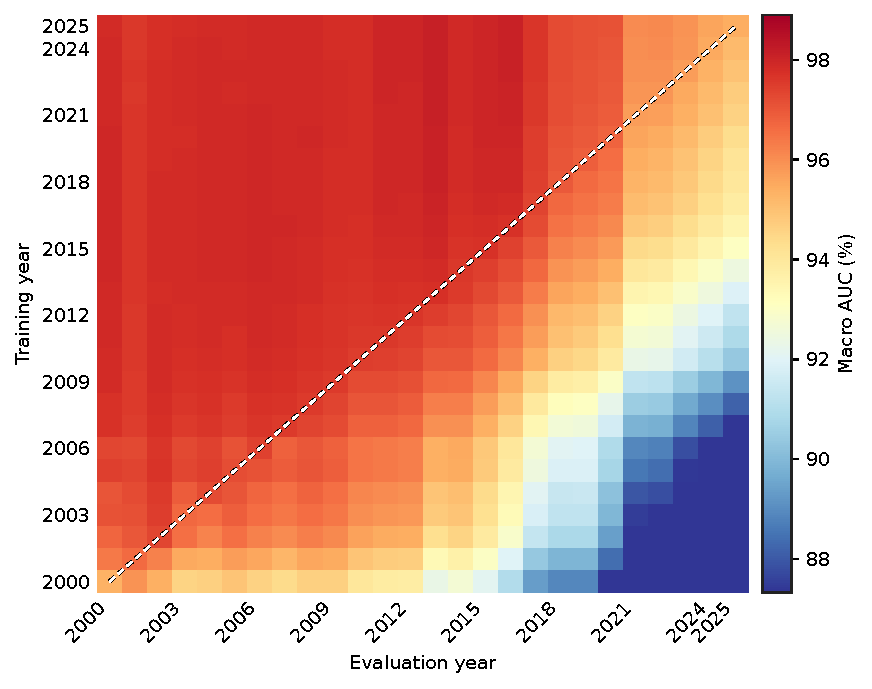
\includegraphics[width=0.5\textwidth]{plots_experiments/arxiv/mean_auc_matrix.pdf}
\caption{Cohort-mean Macro AUC matrix $\bar{M}$ over the arXiv models. Cell $(i,j)$ is the mean across those models of the score from training through slice $i$ and evaluating on slice $j$.}
\label{fig:arxiv_mean_matrix}
\end{figure}

\subsection{Model Roster}

\noindent
\begin{minipage}[t]{0.49\linewidth}
\centering
\footnotesize
\captionof{table}{arXiv: models trained from scratch.}
\label{tab:arxiv_roster}
\resizebox{\ifdim\width>\linewidth \linewidth\else\width\fi}{!}{%
\begin{tabular}{l l rr}
\toprule
Model & Family & Trainable & Total \\
\midrule
TX-S & Transformer & 83k & 124.7M \\
TextCNN-S & TextCNN & 89k & 124.7M \\
FFN-S & FFN & 99k & 124.7M \\
BiGRU-S & Recurrent & 100k & 124.7M \\
FFN-M & FFN & 397k & 125.0M \\
TextCNN-M & TextCNN & 462k & 125.1M \\
TX-M & Transformer & 493k & 125.1M \\
BiLSTM-M & Recurrent & 537k & 125.2M \\
FFN-L & FFN & 1.6M & 126.2M \\
TX-L & Transformer & 1.9M & 126.5M \\
TextCNN-L & TextCNN & 1.9M & 126.6M \\
BiLSTM-Attn-L & Recurrent & 2.2M & 126.8M \\
\bottomrule
\end{tabular}}
\end{minipage}
\hfill
\begin{minipage}[t]{0.49\linewidth}
\centering
\footnotesize
\captionof{table}{arXiv: frozen pretrained encoders, with trainable head and total parameters.}
\label{tab:arxiv_roster_frozen}
\resizebox{\ifdim\width>\linewidth \linewidth\else\width\fi}{!}{%
\begin{tabular}{l l rr}
\toprule
Model & Family & Trainable & Total \\
\midrule
MiniLM-L6 & Frozen & 3k & 22.7M \\
DistilBERT & Frozen & 5k & 66.4M \\
ELECTRA & Frozen & 5k & 108.9M \\
BERT & Frozen & 5k & 109.5M \\
MPNet & Frozen & 5k & 109.5M \\
RoBERTa & Frozen & 5k & 124.7M \\
ModernBERT & Frozen & 5k & 149.0M \\
DeBERTa-v3 & Frozen & 5k & 183.8M \\
\bottomrule
\end{tabular}}
\end{minipage}


\subsection{FFN}

\begin{figure}[H]
\centering
\begin{subfigure}[t]{0.49\textwidth}\centering
    
\includegraphics[width=0.49\linewidth]{plots_experiments/arxiv/raw/FFN-S_drift_matrix.pdf}\hfill
    
\includegraphics[width=0.49\linewidth]{plots_experiments/arxiv/deviation/FFN-S_deviation.pdf}
    \caption{FFN-S}
    \label{fig:arxiv_FFN_S}
\end{subfigure}
\hfill
\begin{subfigure}[t]{0.49\textwidth}\centering
    
\includegraphics[width=0.49\linewidth]{plots_experiments/arxiv/raw/FFN-M_drift_matrix.pdf}\hfill
    
\includegraphics[width=0.49\linewidth]{plots_experiments/arxiv/deviation/FFN-M_deviation.pdf}
    \caption{FFN-M}
    \label{fig:arxiv_FFN_M}
\end{subfigure}

\begin{subfigure}[t]{0.49\textwidth}\centering
    
\includegraphics[width=0.49\linewidth]{plots_experiments/arxiv/raw/FFN-L_drift_matrix.pdf}\hfill
    
\includegraphics[width=0.49\linewidth]{plots_experiments/arxiv/deviation/FFN-L_deviation.pdf}
    \caption{FFN-L}
    \label{fig:arxiv_FFN_L}
\end{subfigure}
\caption{FFN models: Macro AUC drift matrix $M^{(m)}$ and deviation from the cohort mean $\Delta^{(m)} = M^{(m)} - \bar{M}$ for each model, shown on a sequential and a zero-centred diverging scale, respectively.}
\label{fig:arxiv_family_text_ffn}
\end{figure}

\subsection{TextCNN}

\begin{figure}[H]
\centering
\begin{subfigure}[t]{0.49\textwidth}\centering
    
\includegraphics[width=0.49\linewidth]{plots_experiments/arxiv/raw/TextCNN-S_drift_matrix.pdf}\hfill
    
\includegraphics[width=0.49\linewidth]{plots_experiments/arxiv/deviation/TextCNN-S_deviation.pdf}
    \caption{TextCNN-S}
    \label{fig:arxiv_TextCNN_S}
\end{subfigure}
\hfill
\begin{subfigure}[t]{0.49\textwidth}\centering
    
\includegraphics[width=0.49\linewidth]{plots_experiments/arxiv/raw/TextCNN-M_drift_matrix.pdf}\hfill
    
\includegraphics[width=0.49\linewidth]{plots_experiments/arxiv/deviation/TextCNN-M_deviation.pdf}
    \caption{TextCNN-M}
    \label{fig:arxiv_TextCNN_M}
\end{subfigure}

\begin{subfigure}[t]{0.49\textwidth}\centering
    
\includegraphics[width=0.49\linewidth]{plots_experiments/arxiv/raw/TextCNN-L_drift_matrix.pdf}\hfill
    
\includegraphics[width=0.49\linewidth]{plots_experiments/arxiv/deviation/TextCNN-L_deviation.pdf}
    \caption{TextCNN-L}
    \label{fig:arxiv_TextCNN_L}
\end{subfigure}
\caption{TextCNN models: Macro AUC drift matrix $M^{(m)}$ and deviation from the cohort mean $\Delta^{(m)} = M^{(m)} - \bar{M}$ for each model, shown on a sequential and a zero-centred diverging scale, respectively.}
\label{fig:arxiv_family_text_textcnn}
\end{figure}

\subsection{Recurrent}

\begin{figure}[H]
\centering
\begin{subfigure}[t]{0.49\textwidth}\centering
    
\includegraphics[width=0.49\linewidth]{plots_experiments/arxiv/raw/BiGRU-S_drift_matrix.pdf}\hfill
    
\includegraphics[width=0.49\linewidth]{plots_experiments/arxiv/deviation/BiGRU-S_deviation.pdf}
    \caption{BiGRU-S}
    \label{fig:arxiv_BiGRU_S}
\end{subfigure}
\hfill
\begin{subfigure}[t]{0.49\textwidth}\centering
    
\includegraphics[width=0.49\linewidth]{plots_experiments/arxiv/raw/BiLSTM-M_drift_matrix.pdf}\hfill
    
\includegraphics[width=0.49\linewidth]{plots_experiments/arxiv/deviation/BiLSTM-M_deviation.pdf}
    \caption{BiLSTM-M}
    \label{fig:arxiv_BiLSTM_M}
\end{subfigure}

\begin{subfigure}[t]{0.49\textwidth}\centering
    
\includegraphics[width=0.49\linewidth]{plots_experiments/arxiv/raw/BiLSTM-Attn-L_drift_matrix.pdf}\hfill
    
\includegraphics[width=0.49\linewidth]{plots_experiments/arxiv/deviation/BiLSTM-Attn-L_deviation.pdf}
    \caption{BiLSTM-Attn-L}
    \label{fig:arxiv_BiLSTM_Attn_L}
\end{subfigure}
\caption{Recurrent models: Macro AUC drift matrix $M^{(m)}$ and deviation from the cohort mean $\Delta^{(m)} = M^{(m)} - \bar{M}$ for each model, shown on a sequential and a zero-centred diverging scale, respectively.}
\label{fig:arxiv_family_text_rnn}
\end{figure}

\subsection{Transformer}

\begin{figure}[H]
\centering
\begin{subfigure}[t]{0.49\textwidth}\centering
    
\includegraphics[width=0.49\linewidth]{plots_experiments/arxiv/raw/TX-S_drift_matrix.pdf}\hfill
    
\includegraphics[width=0.49\linewidth]{plots_experiments/arxiv/deviation/TX-S_deviation.pdf}
    \caption{TX-S}
    \label{fig:arxiv_TX_S}
\end{subfigure}
\hfill
\begin{subfigure}[t]{0.49\textwidth}\centering
    
\includegraphics[width=0.49\linewidth]{plots_experiments/arxiv/raw/TX-M_drift_matrix.pdf}\hfill
    
\includegraphics[width=0.49\linewidth]{plots_experiments/arxiv/deviation/TX-M_deviation.pdf}
    \caption{TX-M}
    \label{fig:arxiv_TX_M}
\end{subfigure}

\begin{subfigure}[t]{0.49\textwidth}\centering
    
\includegraphics[width=0.49\linewidth]{plots_experiments/arxiv/raw/TX-L_drift_matrix.pdf}\hfill
    
\includegraphics[width=0.49\linewidth]{plots_experiments/arxiv/deviation/TX-L_deviation.pdf}
    \caption{TX-L}
    \label{fig:arxiv_TX_L}
\end{subfigure}
\caption{Transformer models: Macro AUC drift matrix $M^{(m)}$ and deviation from the cohort mean $\Delta^{(m)} = M^{(m)} - \bar{M}$ for each model, shown on a sequential and a zero-centred diverging scale, respectively.}
\label{fig:arxiv_family_text_tx}
\end{figure}

\subsection{Frozen}

\begin{figure}[H]
\centering
\begin{subfigure}[t]{0.49\textwidth}\centering
    
\includegraphics[width=0.49\linewidth]{plots_experiments/arxiv/raw/BERT_drift_matrix.pdf}\hfill
    
\includegraphics[width=0.49\linewidth]{plots_experiments/arxiv/deviation/BERT_deviation.pdf}
    \caption{BERT}
    \label{fig:arxiv_BERT}
\end{subfigure}
\hfill
\begin{subfigure}[t]{0.49\textwidth}\centering
    
\includegraphics[width=0.49\linewidth]{plots_experiments/arxiv/raw/DistilBERT_drift_matrix.pdf}\hfill
    
\includegraphics[width=0.49\linewidth]{plots_experiments/arxiv/deviation/DistilBERT_deviation.pdf}
    \caption{DistilBERT}
    \label{fig:arxiv_DistilBERT}
\end{subfigure}

\begin{subfigure}[t]{0.49\textwidth}\centering
    
\includegraphics[width=0.49\linewidth]{plots_experiments/arxiv/raw/ELECTRA_drift_matrix.pdf}\hfill
    
\includegraphics[width=0.49\linewidth]{plots_experiments/arxiv/deviation/ELECTRA_deviation.pdf}
    \caption{ELECTRA}
    \label{fig:arxiv_ELECTRA}
\end{subfigure}
\hfill
\begin{subfigure}[t]{0.49\textwidth}\centering
    
\includegraphics[width=0.49\linewidth]{plots_experiments/arxiv/raw/MPNet_drift_matrix.pdf}\hfill
    
\includegraphics[width=0.49\linewidth]{plots_experiments/arxiv/deviation/MPNet_deviation.pdf}
    \caption{MPNet}
    \label{fig:arxiv_MPNet}
\end{subfigure}

\begin{subfigure}[t]{0.49\textwidth}\centering
    
\includegraphics[width=0.49\linewidth]{plots_experiments/arxiv/raw/ModernBERT_drift_matrix.pdf}\hfill
    
\includegraphics[width=0.49\linewidth]{plots_experiments/arxiv/deviation/ModernBERT_deviation.pdf}
    \caption{ModernBERT}
    \label{fig:arxiv_ModernBERT}
\end{subfigure}
\hfill
\begin{subfigure}[t]{0.49\textwidth}\centering
    
\includegraphics[width=0.49\linewidth]{plots_experiments/arxiv/raw/RoBERTa_drift_matrix.pdf}\hfill
    
\includegraphics[width=0.49\linewidth]{plots_experiments/arxiv/deviation/RoBERTa_deviation.pdf}
    \caption{RoBERTa}
    \label{fig:arxiv_RoBERTa}
\end{subfigure}

\begin{subfigure}[t]{0.49\textwidth}\centering
    
\includegraphics[width=0.49\linewidth]{plots_experiments/arxiv/raw/DeBERTa-v3_drift_matrix.pdf}\hfill
    
\includegraphics[width=0.49\linewidth]{plots_experiments/arxiv/deviation/DeBERTa-v3_deviation.pdf}
    \caption{DeBERTa-v3}
    \label{fig:arxiv_DeBERTa_v3}
\end{subfigure}
\hfill
\begin{subfigure}[t]{0.49\textwidth}\centering
    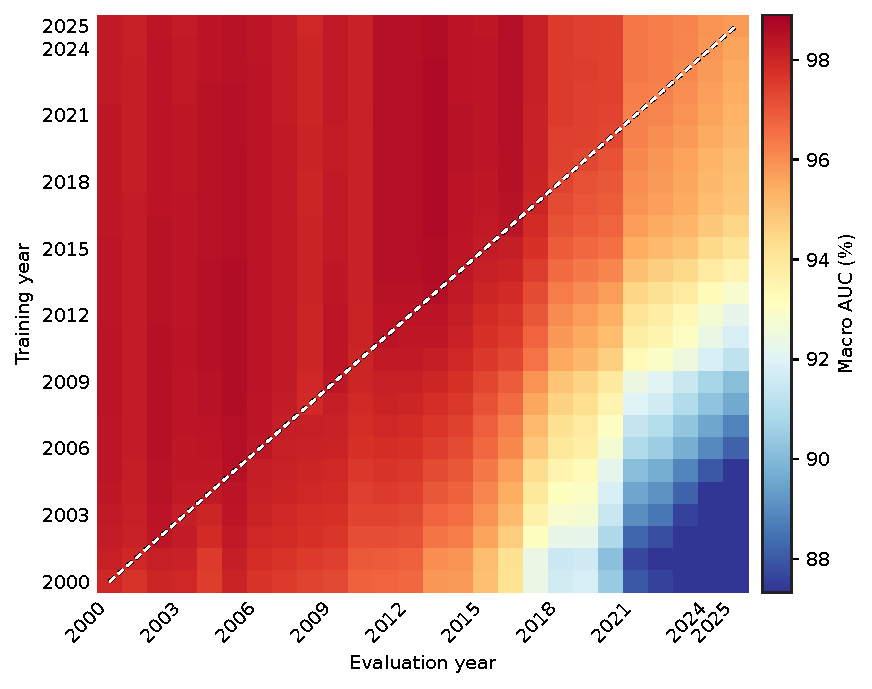
\includegraphics[width=0.49\linewidth]{plots_experiments/arxiv/raw/MiniLM-L6_drift_matrix.pdf}\hfill
    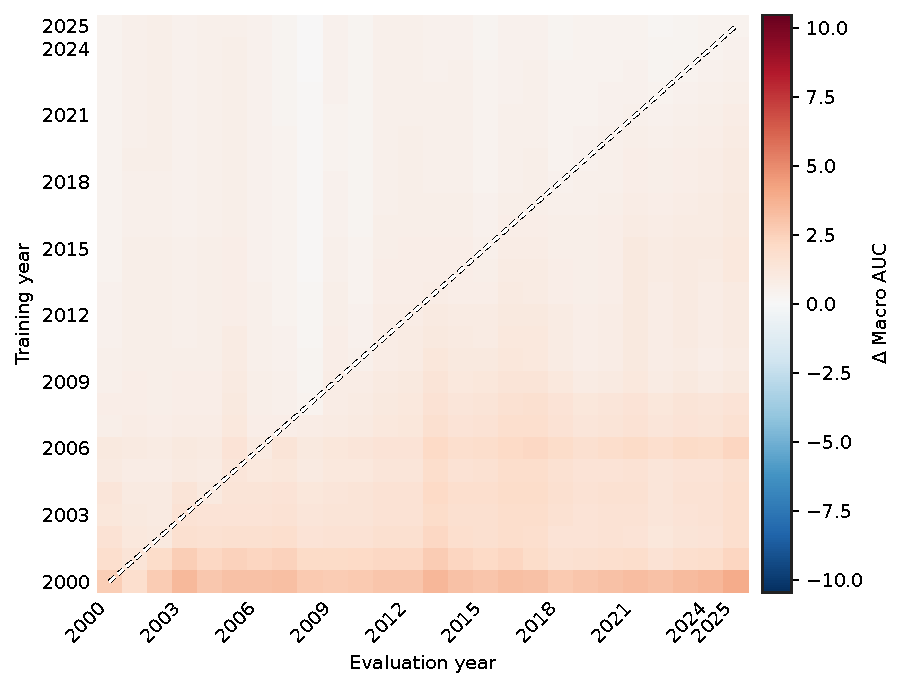
\includegraphics[width=0.49\linewidth]{plots_experiments/arxiv/deviation/MiniLM-L6_deviation.pdf}
    \caption{MiniLM-L6}
    \label{fig:arxiv_MiniLM_L6}
\end{subfigure}
\caption{Frozen models: Macro AUC drift matrix $M^{(m)}$ and deviation from the cohort mean $\Delta^{(m)} = M^{(m)} - \bar{M}$ for each model, shown on a sequential and a zero-centred diverging scale, respectively.}
\label{fig:arxiv_family_text_frozen_head}
\end{figure}

\subsection{Forgetting and Rankings}
\label{app:arxiv_forgetting}

\noindent To see how quickly each model forgets, we summarize its drift matrix as a forgetting curve. The curve plots the Macro AUC against the lag $\ell = j - i$, the number of slices between the training cutoff $i$ and the evaluation slice $j$. At each lag we average over all training cutoffs,
\[ F(\ell) = \operatorname{mean}_{i} M_{i,\,i+\ell}. \]
The result is the Macro AUC at a fixed temporal distance, independent of which period a model was trained on. This separates the effect of temporal distance from the difficulty of any single slice.

\begin{figure}[H]
\centering
\begin{subfigure}[t]{0.49\textwidth}\centering
    
\includegraphics[width=\linewidth]{plots_experiments/arxiv/forgetting.pdf}
    \caption{Per model}
    \label{fig:arxiv_forgetting}
\end{subfigure}\hfill
\begin{subfigure}[t]{0.49\textwidth}\centering
    
\includegraphics[width=\linewidth]{plots_experiments/arxiv/forgetting_by_family.pdf}
    \caption{Per model family}
    \label{fig:arxiv_forgetting_family}
\end{subfigure}
\caption{Forgetting curves: each model (left) and averaged within each family (right).}
\label{fig:arxiv_forgetting_combined}
\end{figure}

\begin{figure}[H]
\centering
\begin{subfigure}[t]{0.49\textwidth}\centering
    
\includegraphics[width=\linewidth]{plots_experiments/arxiv/ranking_future_performance.pdf}
    \caption{By future performance}
    \label{fig:arxiv_ranking_future}
\end{subfigure}\hfill
\begin{subfigure}[t]{0.49\textwidth}\centering
    
\includegraphics[width=\linewidth]{plots_experiments/arxiv/ranking_decay.pdf}
    \caption{By decay}
    \label{fig:arxiv_ranking_decay}
\end{subfigure}
\caption{Models ranked by mean future performance and by temporal decay.}
\label{fig:arxiv_rankings}
\end{figure}

\subsection{Result Tables}

\begin{table}[H]
\centering
\footnotesize
\caption{Temporal robustness on arXiv.}
\label{tab:robustness_arxiv}
\begin{minipage}[t]{0.49\linewidth}
\centering
\resizebox{\ifdim\width>\linewidth \linewidth\else\width\fi}{!}{%
\begin{tabular}{l rr}
\toprule
Model & Future (\%) & Decay (\%) \\
\midrule
ModernBERT & 94.9 & 2.5 \\
FFN-L & 94.9 & 2.7 \\
TextCNN-L & 95.2 & 2.7 \\
TX-M & 95.1 & 2.8 \\
MiniLM-L6 & 94.8 & 2.8 \\
FFN-M & 94.6 & 2.9 \\
TX-S & 95.1 & 2.9 \\
BiLSTM-Attn-L & 95.1 & 2.9 \\
BiLSTM-M & 95.2 & 2.9 \\
TextCNN-M & 94.8 & 3.1 \\
\bottomrule
\end{tabular}}
\end{minipage}\hfill
\begin{minipage}[t]{0.49\linewidth}
\centering
\resizebox{\ifdim\width>\linewidth \linewidth\else\width\fi}{!}{%
\begin{tabular}{l rr}
\toprule
Model & Future (\%) & Decay (\%) \\
\midrule
BERT & 93.6 & 3.1 \\
TX-L & 94.7 & 3.1 \\
BiGRU-S & 94.7 & 3.2 \\
DistilBERT & 93.1 & 3.3 \\
FFN-S & 93.9 & 3.4 \\
TextCNN-S & 94.5 & 3.4 \\
RoBERTa & 92.3 & 3.6 \\
MPNet & 92.0 & 3.7 \\
DeBERTa-v3 & 86.1 & 6.5 \\
ELECTRA & 84.4 & 7.3 \\
\bottomrule
\end{tabular}}
\end{minipage}
\end{table}


\noindent
\begin{minipage}[t]{0.49\linewidth}
\centering
\scriptsize
\setlength{\tabcolsep}{4pt}
\captionof{table}{arXiv: models trained up to 2000, ordered by future performance.}
\label{tab:arxiv_cutoff_2000}
\resizebox{\ifdim\width>\linewidth \linewidth\else\width\fi}{!}{%
\begin{tabular}{c l rrr}
\toprule
Rank & Model & Macro AUC (\%) & Future (\%) & Decay (\%) \\
\midrule
1 & MiniLM-L6 & 97.9 & 93.9 & 4.0 \\
2 & ModernBERT & 97.5 & 93.9 & 3.7 \\
3 & TextCNN-L & 98.1 & 93.8 & 4.3 \\
4 & TX-M & 96.2 & 93.6 & 2.7 \\
5 & BiLSTM-Attn-L & 97.8 & 93.5 & 4.3 \\
6 & TX-S & 96.6 & 93.5 & 3.2 \\
7 & TX-L & 96.2 & 93.4 & 2.8 \\
8 & TextCNN-M & 97.7 & 93.4 & 4.3 \\
9 & FFN-L & 97.2 & 93.2 & 4.0 \\
10 & TextCNN-S & 97.4 & 93.0 & 4.4 \\
11 & BiLSTM-M & 97.3 & 92.8 & 4.5 \\
12 & FFN-M & 96.6 & 92.3 & 4.3 \\
13 & BiGRU-S & 93.3 & 91.9 & 1.4 \\
14 & FFN-S & 95.9 & 91.3 & 4.6 \\
15 & BERT & 95.8 & 90.9 & 4.9 \\
16 & DistilBERT & 94.6 & 90.2 & 4.4 \\
17 & RoBERTa & 91.5 & 88.0 & 3.5 \\
18 & MPNet & 88.9 & 87.3 & 1.6 \\
19 & DeBERTa-v3 & 90.7 & 81.2 & 9.5 \\
20 & ELECTRA & 88.9 & 77.3 & 11.7 \\
\bottomrule
\end{tabular}}
\end{minipage}
\hfill
\begin{minipage}[t]{0.49\linewidth}
\centering
\scriptsize
\setlength{\tabcolsep}{4pt}
\captionof{table}{arXiv: models trained up to 2008, ordered by future performance.}
\label{tab:arxiv_cutoff_2008}
\resizebox{\ifdim\width>\linewidth \linewidth\else\width\fi}{!}{%
\begin{tabular}{c l rrr}
\toprule
Rank & Model & Macro AUC (\%) & Future (\%) & Decay (\%) \\
\midrule
1 & TX-M & 98.6 & 96.0 & 2.6 \\
2 & TextCNN-L & 98.7 & 95.7 & 3.0 \\
3 & BiLSTM-Attn-L & 98.5 & 95.6 & 2.9 \\
4 & BiLSTM-M & 98.8 & 95.6 & 3.2 \\
5 & TX-S & 98.4 & 95.3 & 3.1 \\
6 & FFN-L & 98.0 & 95.2 & 2.8 \\
7 & ModernBERT & 98.0 & 95.0 & 3.0 \\
8 & MiniLM-L6 & 97.9 & 94.9 & 3.0 \\
9 & TextCNN-M & 98.6 & 94.9 & 3.7 \\
10 & FFN-M & 97.9 & 94.9 & 3.0 \\
11 & TX-L & 98.2 & 94.8 & 3.4 \\
12 & BiGRU-S & 98.6 & 94.5 & 4.2 \\
13 & BERT & 97.4 & 93.8 & 3.6 \\
14 & FFN-S & 97.6 & 93.7 & 4.0 \\
15 & TextCNN-S & 98.5 & 93.6 & 4.9 \\
16 & DistilBERT & 97.1 & 93.3 & 3.9 \\
17 & RoBERTa & 96.8 & 92.5 & 4.3 \\
18 & MPNet & 96.7 & 92.5 & 4.3 \\
19 & DeBERTa-v3 & 93.4 & 86.1 & 7.3 \\
20 & ELECTRA & 92.5 & 84.6 & 7.9 \\
\bottomrule
\end{tabular}}
\end{minipage}


\vspace{1.5ex}

\noindent
\begin{minipage}[t]{0.49\linewidth}
\centering
\scriptsize
\setlength{\tabcolsep}{4pt}
\captionof{table}{arXiv: models trained up to 2016, ordered by future performance.}
\label{tab:arxiv_cutoff_2016}
\resizebox{\ifdim\width>\linewidth \linewidth\else\width\fi}{!}{%
\begin{tabular}{c l rrr}
\toprule
Rank & Model & Macro AUC (\%) & Future (\%) & Decay (\%) \\
\midrule
1 & BiLSTM-M & 98.8 & 96.6 & 2.2 \\
2 & BiGRU-S & 98.8 & 96.6 & 2.2 \\
3 & TX-S & 98.7 & 96.5 & 2.2 \\
4 & TX-M & 98.7 & 96.5 & 2.2 \\
5 & TX-L & 98.7 & 96.5 & 2.2 \\
6 & BiLSTM-Attn-L & 98.7 & 96.4 & 2.3 \\
7 & TextCNN-L & 98.6 & 96.3 & 2.3 \\
8 & TextCNN-S & 98.5 & 96.2 & 2.3 \\
9 & TextCNN-M & 98.5 & 96.2 & 2.4 \\
10 & FFN-L & 98.3 & 96.2 & 2.2 \\
11 & FFN-M & 98.2 & 96.1 & 2.2 \\
12 & MiniLM-L6 & 98.4 & 96.0 & 2.4 \\
13 & FFN-S & 98.1 & 96.0 & 2.2 \\
14 & ModernBERT & 98.2 & 95.8 & 2.4 \\
15 & BERT & 97.6 & 95.1 & 2.5 \\
16 & DistilBERT & 97.3 & 94.8 & 2.5 \\
17 & RoBERTa & 97.0 & 94.6 & 2.4 \\
18 & MPNet & 97.0 & 94.4 & 2.5 \\
19 & DeBERTa-v3 & 93.6 & 90.0 & 3.7 \\
20 & ELECTRA & 92.6 & 88.3 & 4.3 \\
\bottomrule
\end{tabular}}
\end{minipage}
\hfill
\begin{minipage}[t]{0.49\linewidth}
\centering
\scriptsize
\setlength{\tabcolsep}{4pt}
\captionof{table}{arXiv: models trained up to 2024, ordered by future performance.}
\label{tab:arxiv_cutoff_2024}
\resizebox{\ifdim\width>\linewidth \linewidth\else\width\fi}{!}{%
\begin{tabular}{c l rrr}
\toprule
Rank & Model & Macro AUC (\%) & Future (\%) & Decay (\%) \\
\midrule
1 & TX-M & 96.5 & 96.3 & 0.1 \\
2 & BiLSTM-M & 96.5 & 96.3 & 0.2 \\
3 & TX-L & 96.4 & 96.3 & 0.2 \\
4 & BiLSTM-Attn-L & 96.4 & 96.3 & 0.2 \\
5 & BiGRU-S & 96.4 & 96.3 & 0.2 \\
6 & TX-S & 96.4 & 96.2 & 0.2 \\
7 & TextCNN-S & 96.2 & 96.0 & 0.2 \\
8 & FFN-L & 96.0 & 95.8 & 0.2 \\
9 & FFN-M & 96.0 & 95.8 & 0.2 \\
10 & TextCNN-M & 96.0 & 95.8 & 0.3 \\
11 & FFN-S & 95.9 & 95.7 & 0.2 \\
12 & MiniLM-L6 & 95.9 & 95.6 & 0.3 \\
13 & TextCNN-L & 95.8 & 95.5 & 0.3 \\
14 & ModernBERT & 95.6 & 95.2 & 0.4 \\
15 & BERT & 95.1 & 94.7 & 0.4 \\
16 & DistilBERT & 94.9 & 94.5 & 0.4 \\
17 & RoBERTa & 94.9 & 94.5 & 0.4 \\
18 & MPNet & 94.9 & 94.4 & 0.4 \\
19 & DeBERTa-v3 & 92.1 & 91.2 & 0.8 \\
20 & ELECTRA & 91.5 & 90.4 & 1.1 \\
\bottomrule
\end{tabular}}
\end{minipage}


\begin{table}[H]
\centering
\footnotesize
\caption{arXiv: future performance and decay by model family.}
\label{tab:arxiv_by_family}
\begin{tabular}{l rrrrrrrr}
\toprule
 & \multicolumn{2}{c}{2000} & \multicolumn{2}{c}{2008} & \multicolumn{2}{c}{2016} & \multicolumn{2}{c}{2024} \\
Family & Future & Decay & Future & Decay & Future & Decay & Future & Decay \\
\midrule
FFN & 92.2 & 4.3 & 94.6 & 3.3 & 96.1 & 2.2 & 95.8 & 0.2 \\
Frozen & 87.8 & 5.4 & 91.6 & 4.6 & 93.6 & 2.8 & 93.8 & 0.5 \\
Recurrent & 92.7 & 3.4 & 95.2 & 3.4 & 96.5 & 2.2 & 96.3 & 0.2 \\
TextCNN & 93.4 & 4.3 & 94.7 & 3.9 & 96.2 & 2.3 & 95.8 & 0.3 \\
Transformer & 93.5 & 2.9 & 95.4 & 3.0 & 96.5 & 2.2 & 96.3 & 0.2 \\
\bottomrule
\end{tabular}
\end{table}

